\begin{figure}[H]
    \centering
    \vskip -\baselineskip
    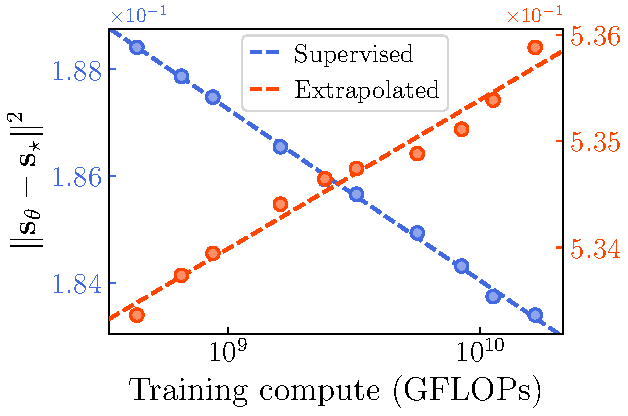
\includegraphics[width=\textwidth,trim={0.2cm 0 0.2cm 0}]{figures/generalization/contrastive_scaling}
    \vskip -0.75\baselineskip
    \caption{\textbf{Quantitative verification of selective underfitting.} $\|\rvs_\theta - \rvs_\star\|^2$ exhibits contrastive scaling behavior in \coloreddashul{xblue}{supervision region} vs.\ \coloreddashul{xred}{extrapolation region}.}
    \label{fig:contrastive-scaling}
\end{figure}